\documentclass[twoside]{article}
\input{ISC18-english.sty}
%%%%%%%%%%%%%%%%%%%%%%%%%%%%  Make sure to compile twice for proper cross-references. %%%%%%%%%%%%%%%%%%%%%%%
%%%%%%% For proper display of references, compile the document twice. %%%%%%%%%%%%%%%%%%%%% 
%%%%%%%%%%%%%%% If using TeX Live, compile using pdflatex command %%%%%%%%%%%%%%%%%%%%%%%
\begin{document}
\thispagestyle{empty}
%%%%%%%%%%%%%%%%% Article title header  %%%%%%%%%%%%%%%%%%%%
\fancyhead[LE]{Cardiovascular Diseases classification}
%%%%%%%%%%%%%%%%% Article authors header   %%%%%%%%%%%%%%%%%%%%
\fancyhead[RO]{Azarnavid, Emami, Abdolhosseinzadeh}
\begin{center}
{
\includegraphics [height=25mm, width=150.3mm] {Images/isc18E}} \\
\vspace*{-1.8cm}
%\begin{center}
%\color{blue} 
%{\hspace{0.1cm}\rule{\textwidth}{1mm}}\\
%\end{center}
\vspace*{4cm}
%%%%%%%%%%%%%%%%% Article title  %%%%%%%%%%%%%%%%%%%%
{\Large \bf Cardiovascular Diseases classification using machine learning models}\\
%%%%%%%%%%%%%%%%% Article authors and affiliations %%%%%%%%%%%%%%%%%%%%
{\bf
Babak Azarnavid\footnote[1]{{\bf Corresponding Author:} {\tt babakazarnavid@ubonab.ac.ir }}, Hojjat Emami$^2$, Mohsen Abdolhosseinzadeh$^3$ \\
$^1$ Department of Mathematics and computer science, Basic Science Faculty, University of Bonab, Bonab, Iran \\
$^2$ Department of Computer Engineering, Faculty of Engineering, University of Bonab, Bonab, Iran \\
$^3$ Department of Mathematics and computer science, Basic Science Faculty, University of Bonab, Bonab, Iran}
\end{center}
\rule{\textwidth}{0.2mm}\\
%%%%%%%%%%%%%%%%% Article abstract  %%%%%%%%%%%%%%%%%%%%
\noindent{\bf Abstract:}\\
Early detection of cardiovascular diseases (CVD) is vital for mitigating mortality and enhancing patient outcomes. Therefore, there is a pressing need for accurate and reliable diagnostic tools. To address this, we evaluated five machine learning models for heart disease prediction: LightGBM, XGBoost, random forest, logistic regression, and a deep neural network. We applied these models to a clinical dataset comprising 1000 patient records. Our experimental results demonstrate that LightGBM achieved the best performance, with a test accuracy of 0.995, a perfect recall score, and an F1 score of 0.996. Finally, SHAP analysis identified slope, resting blood pressure, and serum cholesterol as the most influential predictors in the dataset.
 
\noindent{\bf Keywords:} 
Cardiovascular diseases, Machine learning, Classification, LightGBM\\
\noindent{\bf Mathematics Subject Classification (2010):} $\rm 68T05$, $\rm 62H30$, $\rm 62P10$. \\
\hspace{1cm}\rule{\textwidth}{0.2mm}\\
%%%%%%%%%%%%%%


\section{Introduction}
Cardiovascular diseases (CVDs) remain the leading cause of mortality worldwide, encompassing disorders such as angina pectoris, acute myocardial infarction, and cardiac ischemia. Key risk factors include unhealthy diets, sedentary lifestyles, smoking, uncontrolled blood pressure, and elevated cholesterol. Since heart disease often progresses asymptomatically, early diagnosis is critical to preventing severe outcomes like heart attacks and strokes. However, conventional diagnostic tools—electrocardiograms, stress tests, and coronary angiography—are time‑consuming, costly, and prone to interpretive error. Moreover, they are particularly ineffective in the earliest, asymptomatic stages of the disease. To address this gap, artificial intelligence and machine learning offer a promising alternative, as they can process large clinical datasets and uncover subtle, non‑linear patterns that are difficult for humans to detect. In this study, we develop an early predictive model for heart disease using four machine learning algorithms: LightGBM, XGBoost, Random Forest, and a Multilayer Perceptron (MLP) neural network. By applying these models to clinical data, we aim to build a reliable, accurate decision‑support system that can assist healthcare professionals in achieving timely diagnoses and tailoring personalized treatment plans.

\section{Related Work}
In recent years, numerous studies have used machine learning techniques for predicting and diagnosing heart disease. In this section, we review key studies that are methodologically or dataset-wise aligned with the present research. Santhosh et al. \cite{Santhosh2025} used machine learning algorithms such as Random Forest, Logistic Regression, KNN, and XGBoost to analyze cardiac data from a multi-specialty hospital in India. By using a model stacking technique, they developed a model called CARDIACX and achieved an accuracy of 98.5\% and an area under the curve (AUC) of 0.99 using explainable artificial intelligence (XAI) methods such as SHAP and LIME. Ali et al. \cite{Ali2021} showed through supervised learning that Random Forest can achieve very high accuracies in clinical applications. Doppala et al. \cite{Doppala2022} presented a reliable Ensemble Model based on a voting mechanism, combining Naïve Bayes, Random Forest, SVM, and XGBoost. Their model achieved an accuracy of 96.75\% on the Mendeley dataset. Sonawane and Patil \cite{Sonawane2014} used a Multilayer Perceptron (MLP) and reported 98\% accuracy in predicting coronary artery disease. Sivakami et al. \cite{Sivakami2026} proposed a decentralized framework called DFBCI based on federated learning, blockchain, and quantum cryptography. Using Federated Dynamic Relational Learning (FDRL) and deep neural networks, they analyzed multi-modal data such as ECG and biomarkers, which led to a 19\% improvement in cardiac risk classification. Rehman et al. \cite{Rehman2022}, used a combination of federated learning and Deep Extreme Learning Machine (DELM) networks for disease prediction. Aradhya et al. \cite{Manjunath2024} examined the challenge of learning with limited data. By combining two datasets, including Mendeley data, they showed that ensemble models such as Bagged Ensemble and Sparse SVM remain highly stable and accurate even with a very small amount of training data (for example, only two samples), and they reached an accuracy of 86.69\%. Mienye and Jere \cite{Mienye2024} proposed an optimized ensemble learning model based on the combination of AdaBoost, Random Forest, and XGBoost models for heart disease prediction, which utilizes Bayesian optimization for hyperparameter tuning and SHAP for model interpretability. David in \cite{David2021} focused on the role of cardiac biomarkers such as troponin-I and CK-MB in the early diagnosis of myocardial infarction. They designed a super learner model, using a combination of Decision Tree and CatBoost as base models and Logistic Regression as the meta-learner, which achieved 97.9\% accuracy on biomarker data and 98.8\% on the Mendeley dataset. This use of meta-learners is consistent with the idea of Weng et al. \cite{Weng2017}, who showed that neural networks and Gradient Boosting Machines (GBM) perform better in identifying high-risk patients. Inspired by the success of ML methods in the studies above, the present research examines several ML models including LightGBM, XGBoost, Random Forest, and neural networks (MLP) to address the cardiovascular diseases classification problem.





%%%%%%%%%%%%%%%%%%%


\section{Machine learning models}
To thoroughly examine the classification capacity for the CVD problem, this research uses a heterogeneous set of five ML models. This selection was strategically designed to use distinct algorithms, enabling us to conduct a comparative analysis between traditional statistical methods and recent ensemble algorithms. The evaluated models are logistic regression (LR), random forest (RF), XGBoost, LightGBM, and deep neural network (DNN). LR served as an interpretable, low-cost baseline by calculating the probability of classes via a sigmoid function applied to the linear combination of input features. As a bagging ensemble, RF integrates predictions from multiple decision trees (DT) to decrease variance and offers intrinsic feature importance rankings for clinical interpretability. XGBoost, a well-known gradient-boosting strategy, sequentially modifies prediction residuals with built-in L1/L2 regularization and parallelized tree creation for effective convergence. LightGBM incorporates a leaf-wise tree growth method, integrated with exclusive feature bundling (EFB) and gradient-based one-side sampling (GOSS) to accelerate training and handle high-dimensional medical data while maintaining strong predictive power. DNN was selected to automatically learn hierarchical feature interactions using multiple non-linear hidden layers, while dropout and batch normalization were employed to reduce overfitting and guarantee stable gradient propagation in the training phase.

\section{Experimental results and discussion}
\subsection{Dataset}
The dataset used in this study was obtained from the Mendeley Data scientific repository \cite{Doppala2021}. This data was originally collected from a multispecialty hospital in India. The main strength of this dataset is that it has no missing values and a relatively balanced distribution of the target classes, making it an ideal resource for training powerful machine learning models. It contains 1,000 patient records (subjects) and is statistically considered one of the most comprehensive datasets available for research on the early detection of heart disease. Before public release, all patient records were fully anonymized to protect individuals’ privacy. Each record in this dataset is described using 12 to 14 common clinical features, including demographic characteristics and physiological vital indicators. Table \ref{tbl1} summarizes the characteristics and definitions of all variables included in the dataset.


\begin{table}[]
	\centering
	\label{tbl1}
	\caption{Characteristics of the benchmark dataset}
	\begin{tabular}{lll}
		\hline
		Feature              & Description                                                            & Type    \\ \hline
		Age                  & Age in years                                                           & Numeric \\
		Gender               & Female (0) or male (1)                                                 & Binary  \\
		Chest pain type      & 0: typical angina, 1: atypical angina, 2: non-anginal, 3: asymptomatic & Nominal \\
		Resting BP           & Resting systolic blood pressure (mm Hg)                                & Numeric \\
		Serum cholesterol    & Serum cholesterol (mg/dl)                                              & Numeric \\
		Fasting blood sugar  & \textgreater 120 mg/dl (0: false, 1: true)                             & Binary  \\
		Resting ECG          & 0: normal, 1: ST-T abnormality, 2: LV hypertrophy                      & Nominal \\
		Max heart rate       & Maximum achieved heart rate                                            & Numeric \\
		Exercise angina      & Chest pain during exercise (0: no, 1: yes)                             & Binary  \\
		Oldpeak              & ST depression relative to rest                                         & Numeric \\
		Slope                & 1: upsloping, 2: flat, 3: downsloping                                  & Nominal \\
		No. of major vessels & Number of major vessels (0–3)                                          & Numeric \\
		Target               & 0: no disease, 1: disease present                                      & Binary  \\ \hline
	\end{tabular}
\end{table}

Figure \ref{fig1} illustrates the correlation matrix for the benchmark dataset. The plot reveals that slope (0.80), chest pain type (0.55), number of major vessels (0.49), and resting blood pressure (0.48) have the strongest positive correlations with the target, proving these are the most influential linear predictors in this dataset. In contrast, gender, age, and exercise-angina show weak correlations with the target.

\begin{figure}[ht]
	\begin{center}
		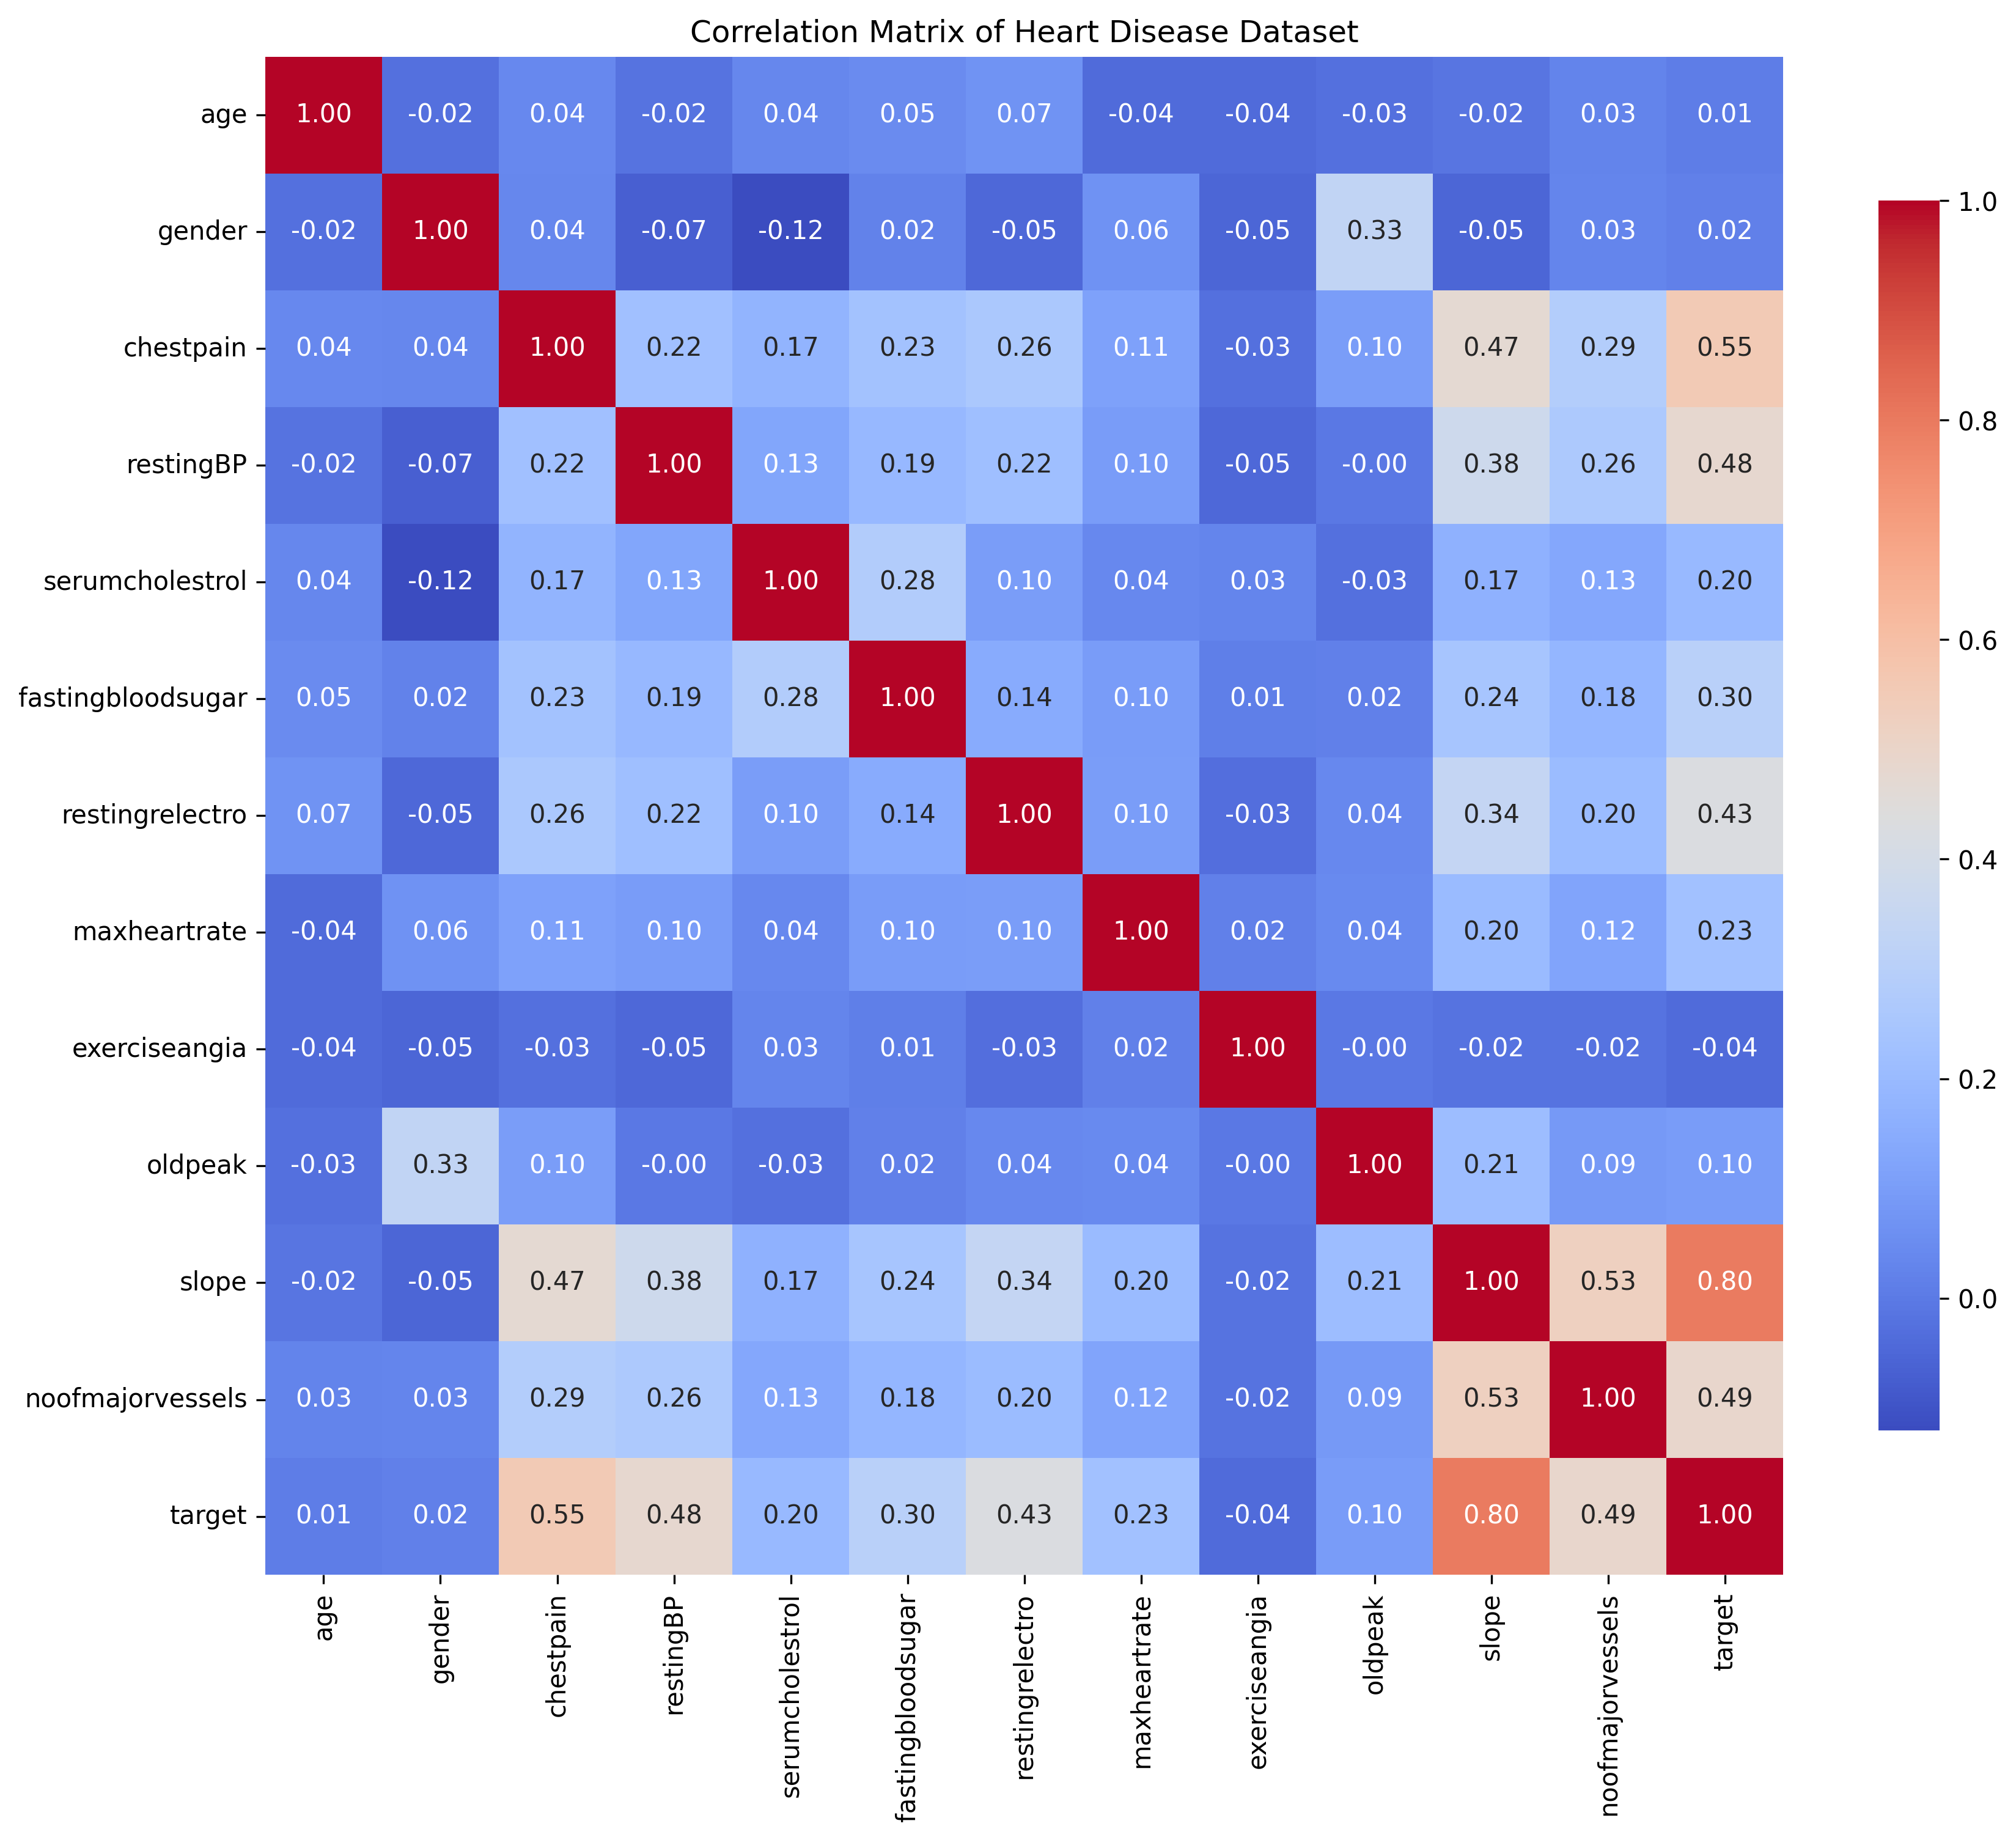
\includegraphics[width=7cm,height=6cm]{correlation_heatmap.png}
		\vspace{-0.2cm}
		\caption{\footnotesize{Correlation matrix of the CVD dataset}}
	\end{center}
\label{fig1}
\end{figure}



\subsection{Performance metrics}
The ML models were evaluated using four metrics, including accuracy, precision, recall, and F1 score. Details of these measures are given in \cite{Sokolova2009}.


\subsection{Statistical results}
Table \ref{tbl2} lists the results generated by predictive algorithms on the benchmark dataset. The results prove that all ML algorithms obtain strong results, with the tree-based ensemble models significantly outperforming the neural network and linear algorithms. Notably, LightGBM, XGBoost, and RF all generated perfect training scores (1.00 across all metrics), while they generalize exceptionally well to unseen test data, with accuracies exceeding 99\%, proving minimal overfitting. Among all models, LightGBM yields the best overall performance, obtaining the highest test accuracy (0.995), F1-score (0.9957), and recall (1.00). This fact proves that LightGBM successfully identified every single positive case without any false negatives. In contrast, LR shows poor results with a test accuracy of 96\% and a decrease in accuracy from 0.972 (training) to 0.950 (test), proving that it produces fewer false positives in the test data. The DNN yields middle performances, indicating solid generalization with a test F1 of 0.9746 and an accuracy of 97\%, but it is finally outperformed by the simple, more powerful ensemble tree models. Overall, the findings clearly prove that the benchmark data is highly separable, and LightGBM is known as a well-balanced and most reliable model for the CVD classification problem. It generated the best trade-off between recall and precision on the testing benchmark. Regarding the performance metrics, the ranking of the models is $ LightGBM> RF > XGBoost> DNN> LR $.



\begin{table}[]
	\caption{Results of ML models on the training and testing datasets}
	\begin{tabular}{lllllllll}
		\hline
		\multirow{2}{*}{Model} & \multicolumn{4}{l}{Training}             & \multicolumn{4}{l}{Testing}              \\ \cline{2-9} 
		& Accuracy & Precision & Recall  & F1      & Accuracy & Precision & Recall  & F1      \\ \hline
		RF                     & 1.00000  & 1.00000   & 1.00000 & 1.00000 & 0.99000  & 0.99138   & 0.99138 & 0.99138 \\
		XGBoost                & 1.00000  & 1.00000   & 1.00000 & 1.00000 & 0.99000  & 0.99138   & 0.99138 & 0.99138 \\
		LightGBM               & 1.00000  & 1.00000   & 1.00000 & 1.00000 & 0.99500  & 0.99145   & 1.00000 & 0.99571 \\
		LR                     & 0.96125  & 0.97168   & 0.96121 & 0.96641 & 0.96000  & 0.95000   & 0.98276 & 0.96610 \\
		DNN                    & 0.98375  & 0.98287   & 0.98922 & 0.98604 & 0.97000  & 0.95833   & 0.99138 & 0.97458 \\ \hline
	\end{tabular}
\label{tbl2}
\end{table}


Figure \ref{fig2} presents the confusion matrix for the ML models, with the y-axis showing the true class and the x-axis the predicted class. Each cell shows the count of actual samples assigned to each predicted class. Diagonal cells indicate correct classifications, while off-diagonal cells indicate misclassifications (false negatives and false positives). The results confirm that the LightGBM model performs strongly and outperforms its counterparts. XGBoost and RF generated the same results. LR obtained the weakest results, and DNN generated moderate results.



\begin{figure}[ht]
	\begin{center}
		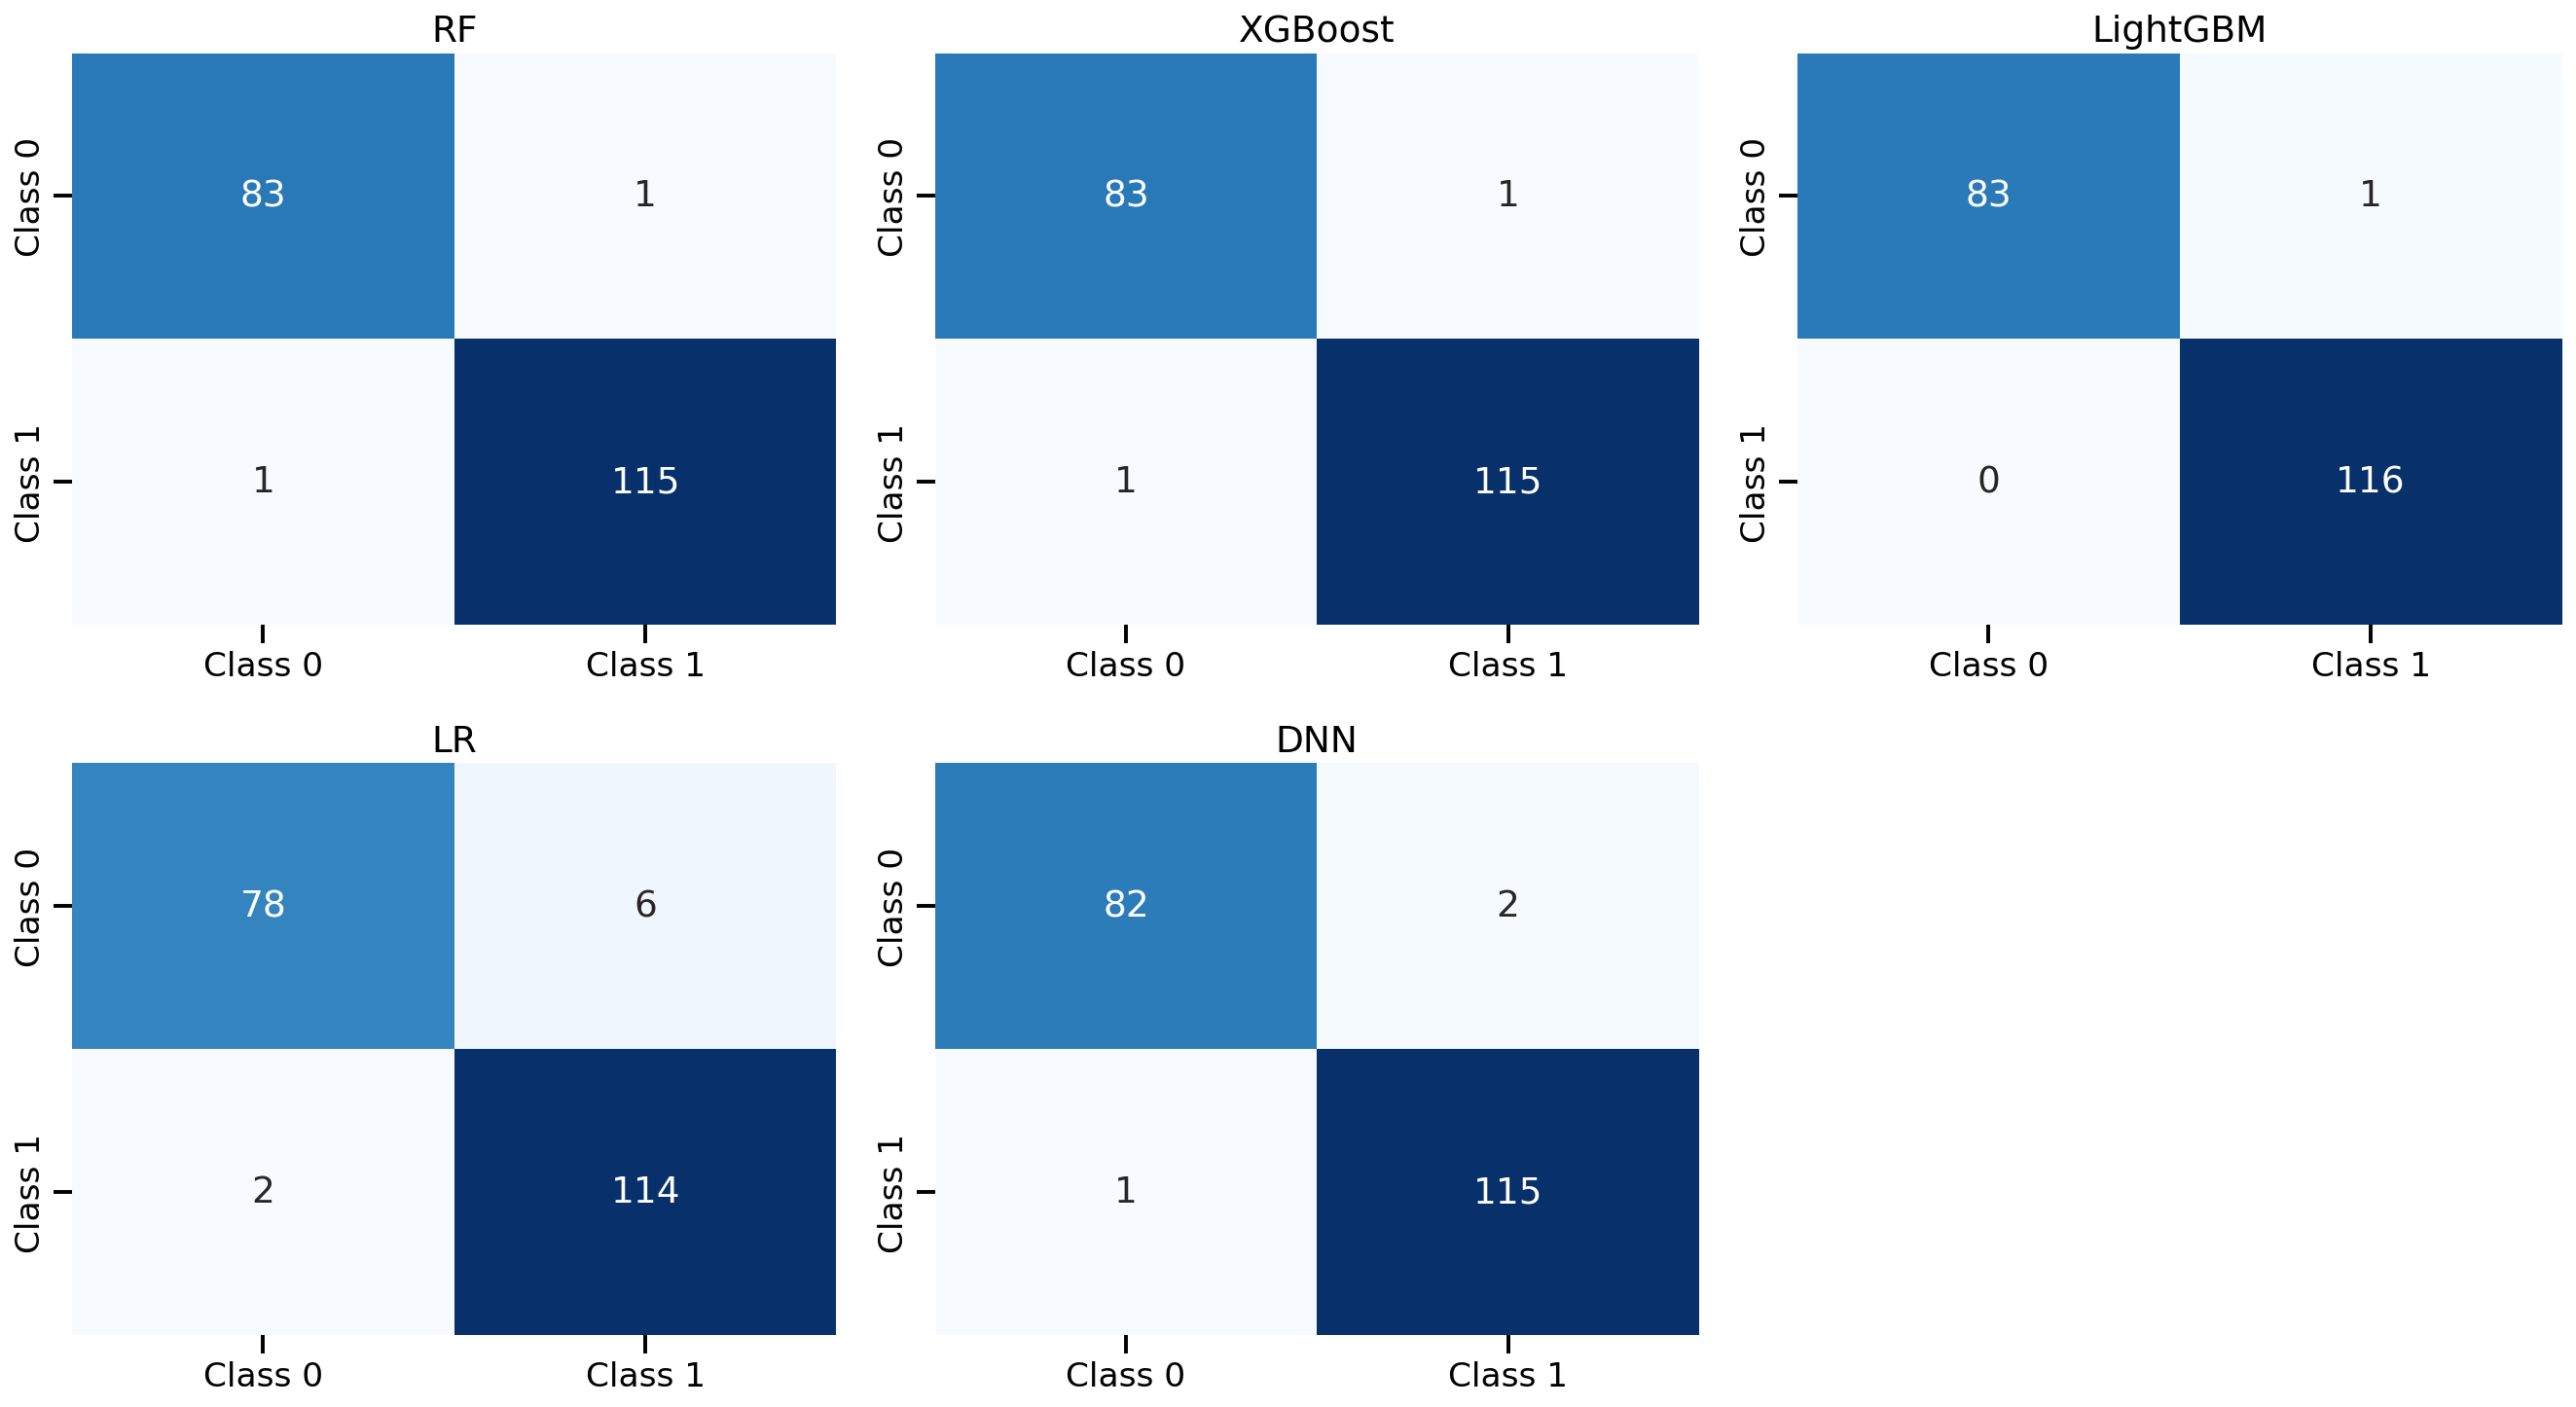
\includegraphics[width=7cm,height=6cm]{combined_confusion_matrices.png}
		\vspace{-0.2cm}
		\caption{\footnotesize{Confusion matrix generated by ML models}}
	\end{center}
\label{fig2}
\end{figure}


Figure \ref{fig3} shows the calibration analysis results for ML models. The plots show that LightGBM, RF, and XGBoost yield near perfect reliability. These minimal errors highlight that the predicted probabilities closely match the observations, confirming that the models are very well calibrated.


\begin{figure}[ht]
	\begin{center}
		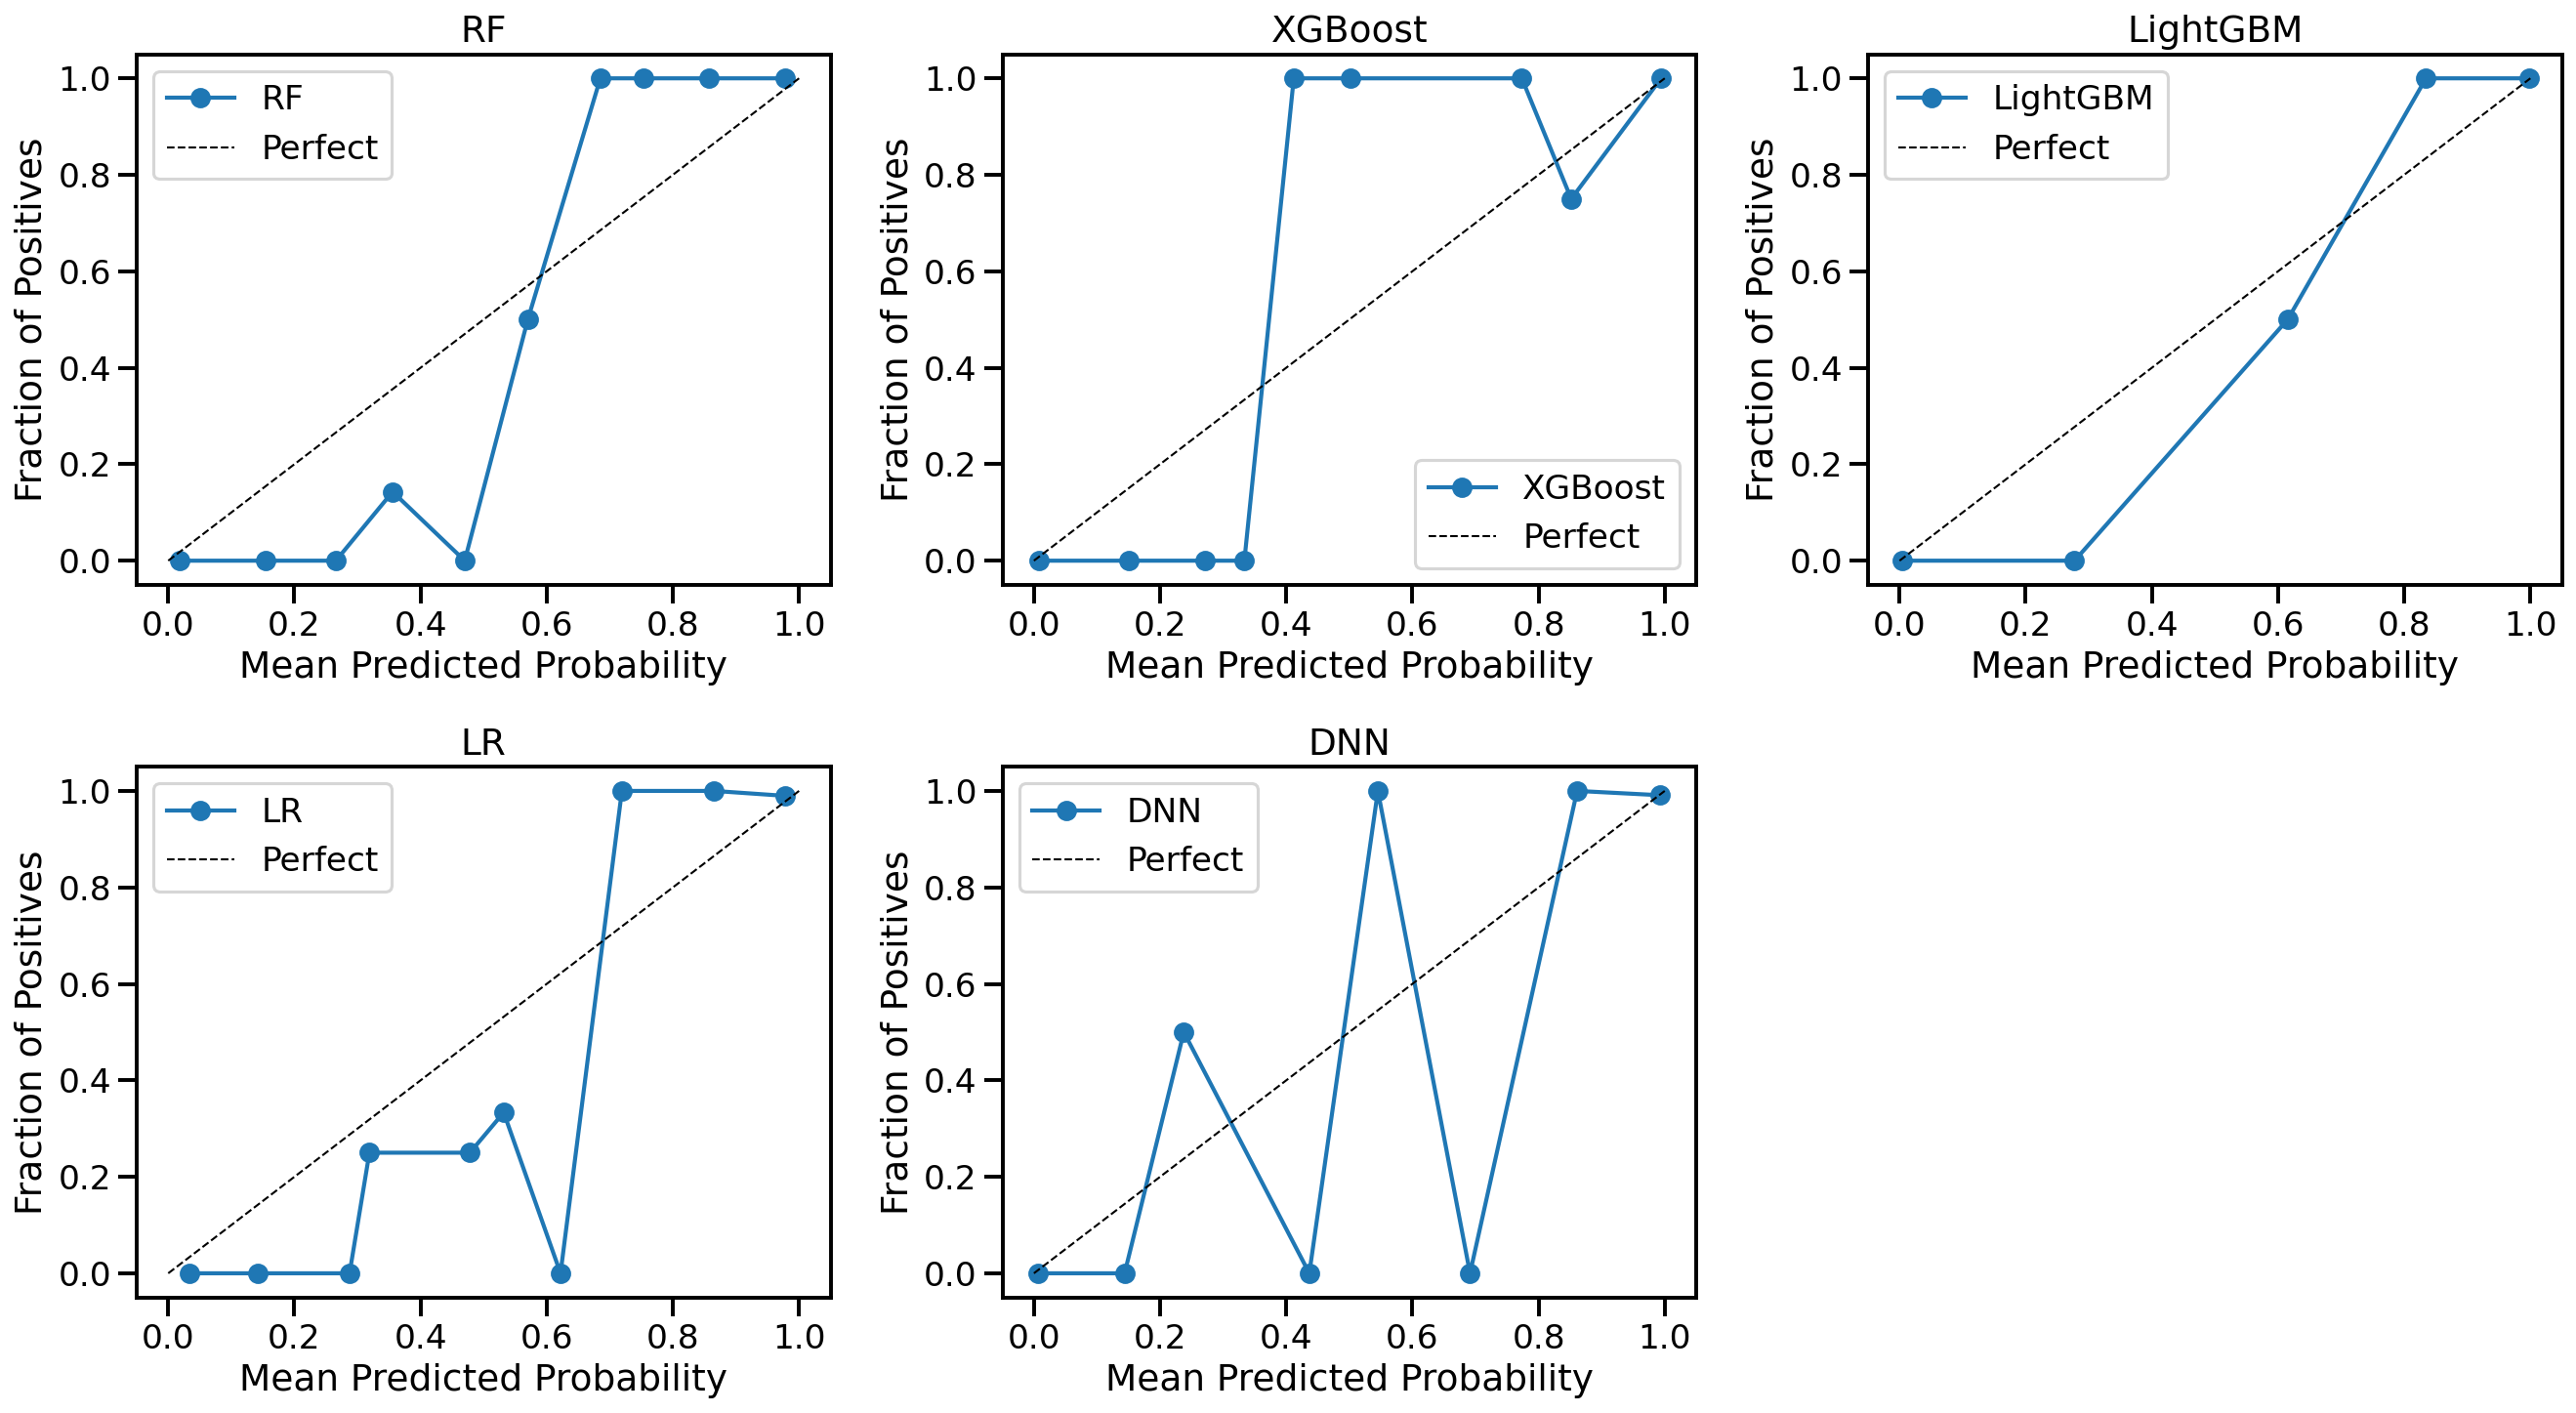
\includegraphics[width=7cm,height=6cm]{combined_calibration_subplots.png}
		\vspace{-0.2cm}
		\caption{\footnotesize{Calibration analysis results for ML models}}
	\end{center}
\label{fig3}
\end{figure}

Figure \ref{fig4} shows the precision-recall and ROC-AUC analysis for ML models. All models show near perfect classification performance, with ROC AUC values ranging from 0.996 to 1.00 and PR AP scores from 0.997 to 1.00, highlighting exceptionally high discriminative ability. XGBoost and LightGBM generate the best scores (AUC = 1.00, AP = 1.00), slightly outperforming the DNN (AUC = 0.998) and LR (AUC = 0.996), proving ensemble tree models are particularly well suited for this dataset.

\begin{figure}[ht]
	\begin{center}
		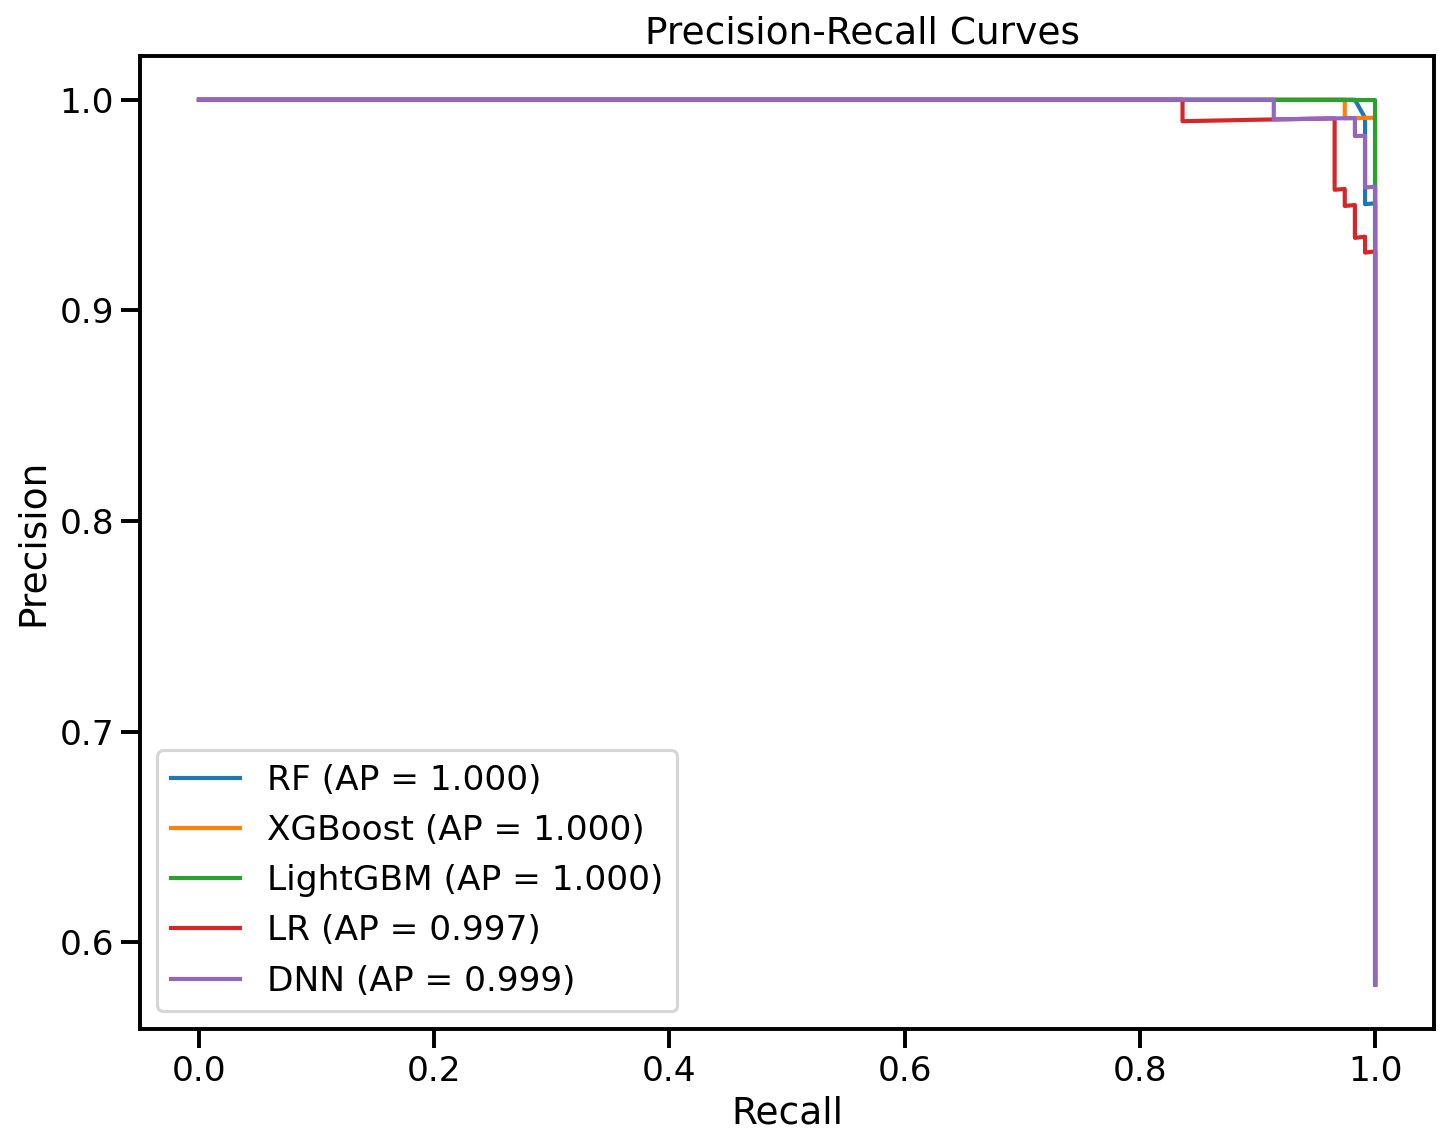
\includegraphics[width=7cm,height=6cm]{combined_pr_curves.png}
		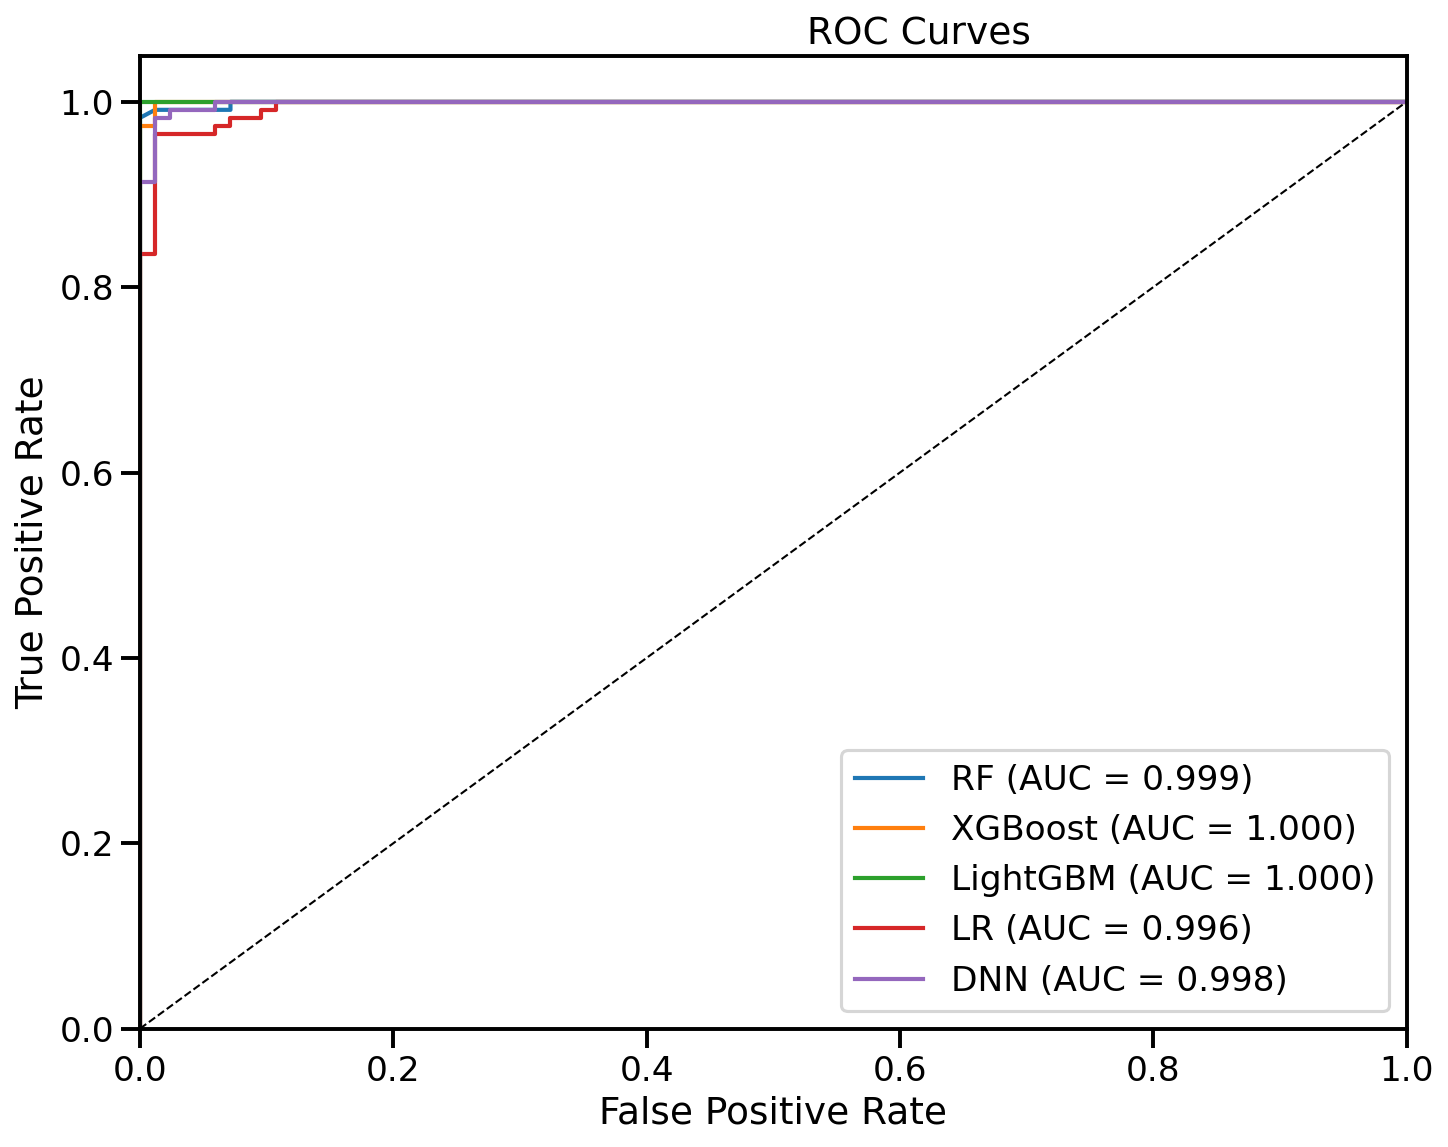
\includegraphics[width=7cm,height=6cm]{combined_roc_curves.png}
		\vspace{-0.2cm}
		\caption{\footnotesize{Precision-recall curves and ROC-AUC analysis of ML models}}
	\end{center}
\label{fig4}
\end{figure}


Figure \ref{fig6} shows the SHAP analysis results generated by the LightGBM model. The SHAP feature importance plot proves that slope, restingBP, and serumcholesterol are the top three most important features. The SHAP summary results show that higher values of slope, restingBP, and chestpain generally push the model toward a higher probability of heart disease, while features like exerciseangia and age show negligible impact on the prediction of disease.

\begin{figure}[ht]
	\begin{center}
		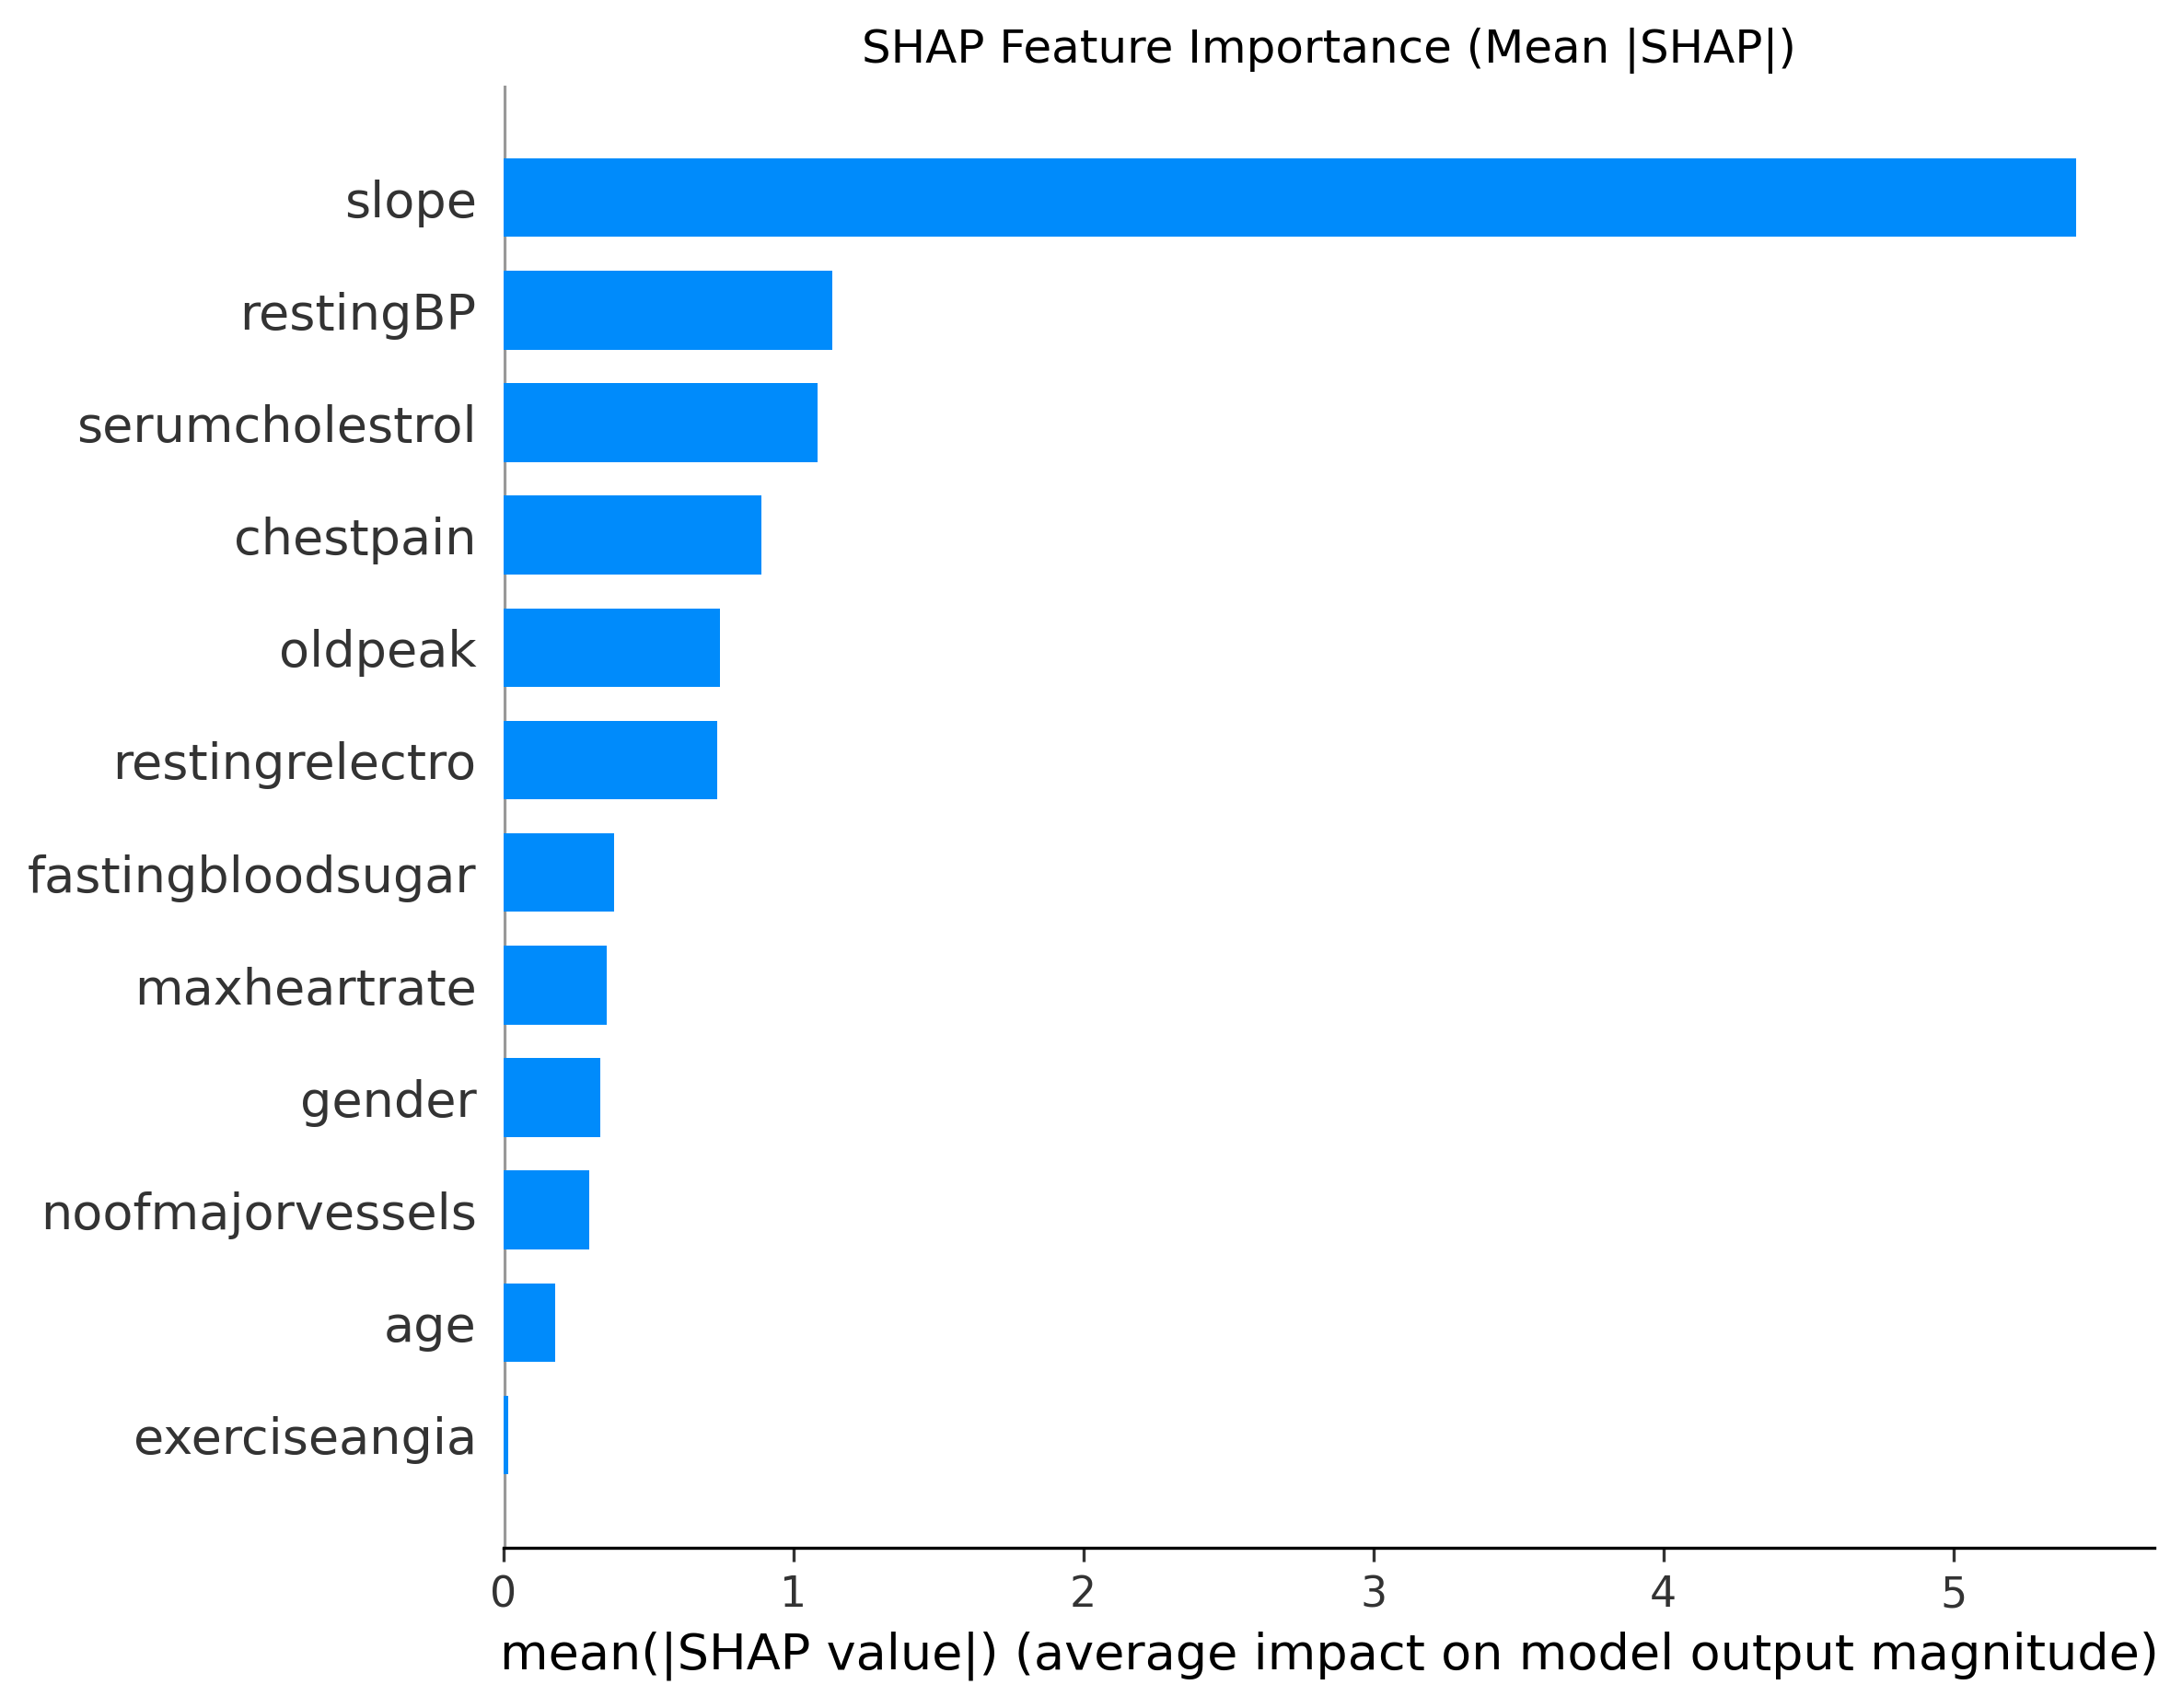
\includegraphics[width=7cm,height=6cm]{shap_bar.png}
		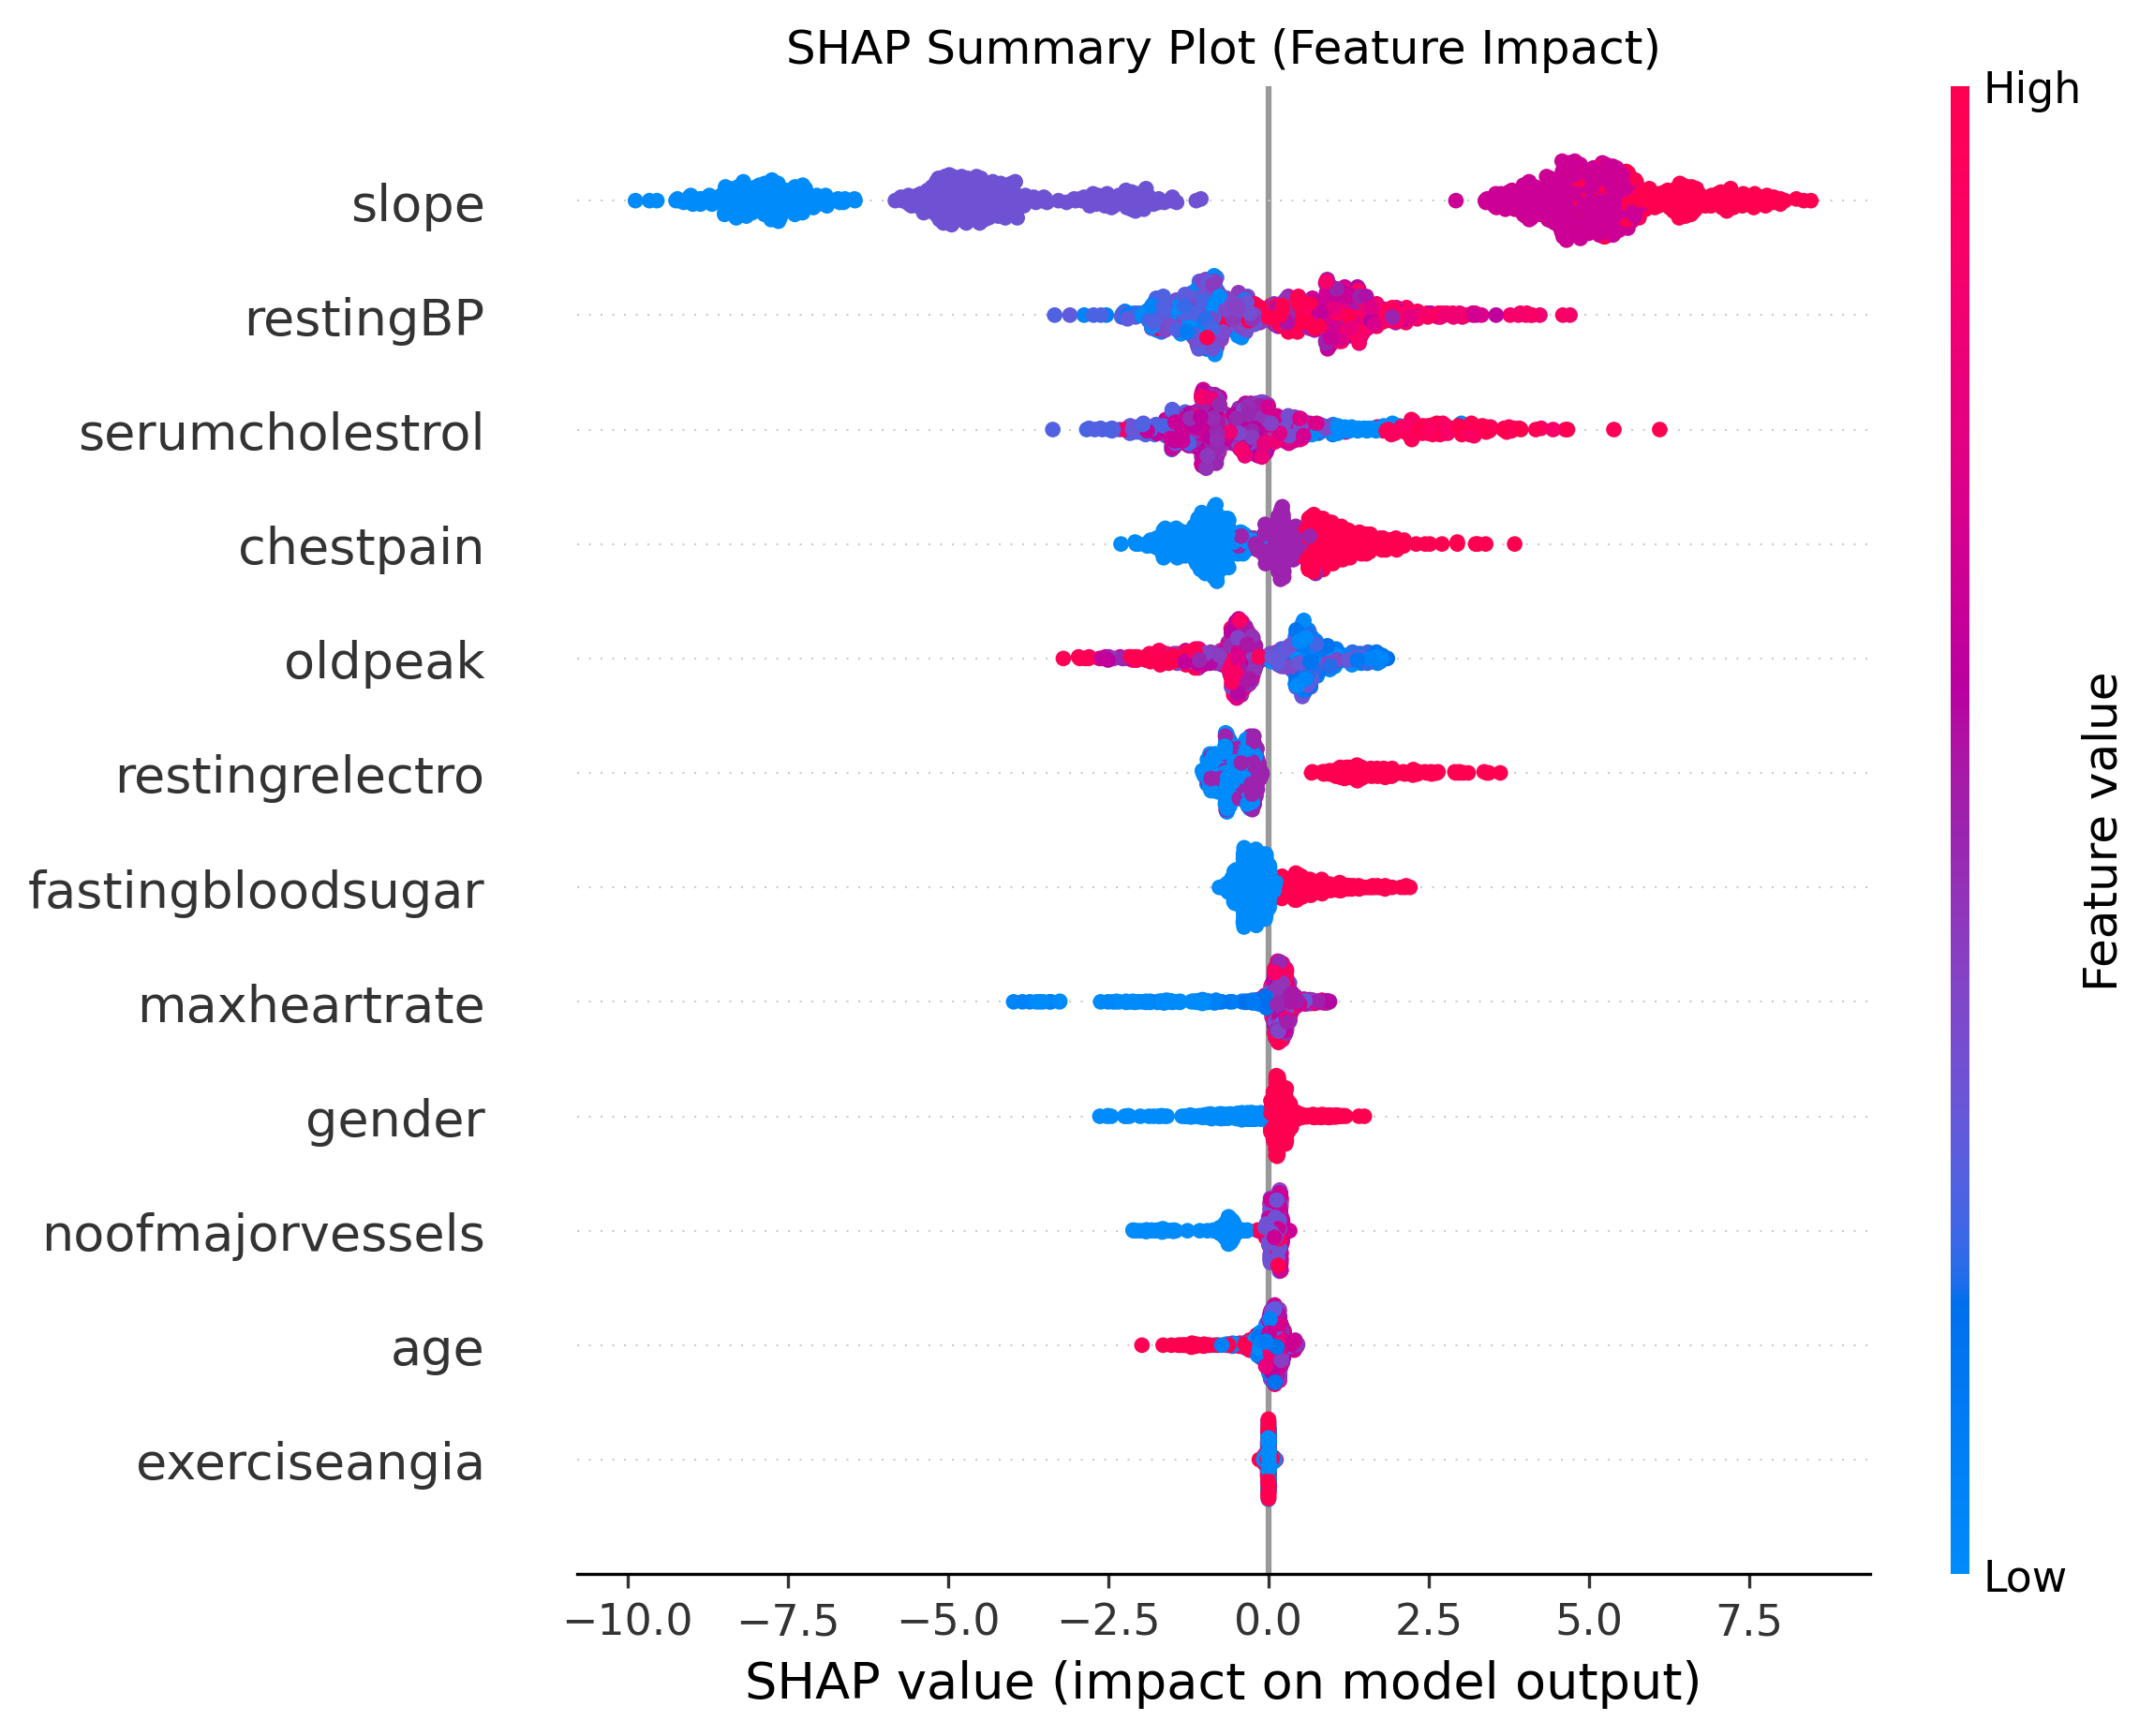
\includegraphics[width=7cm,height=6cm]{shap_summary.png}
		\vspace{-0.2cm}
		\caption{\footnotesize{SHAP analysis results based on the LightGBM model on the benchmark dataset}}
	\end{center}
\label{fig6}
\end{figure}

\section{Conclusion}
In this study, we evaluated five machine learning models—LightGBM, XGBoost, Random Forest, Logistic Regression, and Deep Neural Networks—for classifying cardiovascular disease using a Mendeley clinical dataset of 1,000 patients. Our results demonstrate that tree‑based ensemble models outperformed both linear models and neural networks. Among all models, LightGBM achieved the highest performance, with a test accuracy of 0.995, perfect recall (1.00), and an F1‑score of 0.996, successfully identifying all disease cases without any false negatives. To enhance interpretability, we performed SHAP analysis on the LightGBM model, which identified peak exercise ST segment slope, resting blood pressure, and serum cholesterol as the most significant predictors—findings that align with documented clinical evidence. This transparency supports clinicians in understanding the basis of predictions and making more informed decisions. Overall, our findings underscore the strong potential of gradient‑boosting ensemble models for early CVD detection. However, a key limitation is the reliance on a single‑center dataset, which restricts direct generalizability to more diverse populations. Future research should address this through multi‑center data collection, federated learning approaches, and the development of user‑friendly interfaces for real‑world clinical deployment.


\begin{thebibliography}{9}

\bibitem[Coffey et al. (2021)]{Coffey2021}
Coffey Sean, Roberts-Thomson Ross, Brown Alex, Carapetis Jonathan, Chen Mao, Enriquez-Sarano Maurice, Z\"{u}hlke Liesl, and Prendergast Bernard D. (2021), Global epidemiology of valvular heart disease, {\it Nature Reviews Cardiology} 18, 12, 853-864.

\bibitem[Hanson et al. (2013)]{Hanson2013}
Hanson Michele A., Fareed Mohammad Tariq, Argenio Sandra L., Agunwamba Akochi O., and Hanson Teresa R. (2013), Coronary artery disease, {\it Primary Care} 40, 1, 1-16.

\bibitem[Stamler and Epstein (1972)]{Stamler1972}
Stamler Jeremiah and Epstein Frederick H. (1972), Coronary heart disease: risk factors as guides to preventive action, {\it Preventive Medicine} 1, 1-2, 27-48.


\bibitem[Rajkomar et al. (2019)]{Rajkomar2019}
Rajkomar Alvin, Dean Jeffrey, and Kohane Isaac (2019), Machine learning in medicine, {\it New England Journal of Medicine} 380, 14, 1347-1358.


\bibitem[Santhosh et al. (2025)]{Santhosh2025}
Santhosh Sujith, Chadaga Krishnaraj, Arjunan R. Vijaya, and D'Souza Sandra (2025), Cardiac clarity: Harnessing machine learning for accurate heart-disease prediction, {\it IEEE Access} 13, 97529-97544.
\bibitem[Ali et al. (2021)]{Ali2021}
Ali Md Mamun, Paul Bikash Kumar, Ahmed Kawsar, Bui Francis M., Quinn Julian MW, and Moni Mohammad Ali (2021), Heart disease prediction using supervised machine learning algorithms: Performance analysis and comparison, {\it Computers in Biology and Medicine} 136, 104672.
\bibitem[Doppala et al. (2022)]{Doppala2022}
Doppala Bhanu Prakash, Bhattacharyya Debnath, Janarthanan Midhunchakkaravarthy, and Baik Namkyun (2022), A reliable machine intelligence model for accurate identification of cardiovascular diseases using ensemble techniques, {\it Journal of Healthcare Engineering} 2022, 1, 2585235.

\bibitem[Sonawane and Patil (2014)]{Sonawane2014}
Sonawane Jayshril S. and Patil Dharmaraj R. (2014), Prediction of heart disease using multilayer perceptron neural network, in {\it International Conference on Information Communication and Embedded Systems (ICICES2014)}, pp. 1-6, IEEE.

\bibitem[Sivakami et al. (2026)]{Sivakami2026}
Sivakami R., Kumar V. Vinoth, Krishnamoorthy N., and Yimer Temesgen Engida (2026), Quantum-enhanced federated blockchain for privacy-preserving cardiovascular intelligence, {\it Scientific Reports}.
\bibitem[Rehman et al. (2022)]{Rehman2022}
Rehman Abdur, Abbas Sagheer, Khan M.A., Ghazal Taher M., Adnan Khan Muhammad, and Mosavi Amir (2022), A secure healthcare 5.0 system based on blockchain technology entangled with federated learning technique, {\it Computers in Biology and Medicine} 150, 106019.


\bibitem[Manjunath Aradhya et al. (2024)]{Manjunath2024}
Manjunath Aradhya V. N., Shiva Prasad P., and Chaithra C. S. (2024), Learning with Limited Data: A Machine Learning Approach for Heart Disease Prediction, in {\it International Conference on Current Advancements in Machine Learning}, pp. 1-12, Cham, Springer Nature Switzerland.

\bibitem[Mienye and Jere (2024)]{Mienye2024}
Mienye Ibomoiye Domor and Jere Nobert (2024), Optimized ensemble learning approach with explainable AI for improved heart disease prediction, {\it Information} 15, 7, 394.

\bibitem[David (2021)]{David2021}
David Vasantha Kalyani (2021), Super learner model in prediction of heart attack based on cardiac biomarkers, {\it Indian Journal of Computer Science and Engineering} 12, 6, 1702-1712.
\bibitem[Weng et al. (2017)]{Weng2017}
Weng Stephen F., Reps Jenna, Kai Joe, Garibaldi Jonathan M., and Qureshi Nadeem (2017), Can machine-learning improve cardiovascular risk prediction using routine clinical data?, {\it PLOS ONE} 12, 4, e0174944.



\bibitem[Doppala and Bhattacharyya (2021)]{Doppala2021}
Doppala Bhanu Prakash and Bhattacharyya Debnath (2021), Cardiovascular\_Disease\_Dataset, {\it Mendeley Data} V1, doi: 10.17632/dzz48mvjht.1.



\bibitem[Sokolova and Lapalme (2009)]{Sokolova2009}
Sokolova Marina and Lapalme Guy (2009), A systematic analysis of performance measures for classification tasks, {\it Information Processing \& Management} 45, 4, 427-437.



\end{thebibliography}

%\begin{thebibliography}{9}
%\bibitem[Craik (2005)]{Craik:2005}
%Craik A.D.D. (2005), Prehistory of Fa\`{a} di Bruno's formula, {\it The American Mathematical Monthly} 112, 2,  119-130.
%\bibitem[Feller (1972)]{Feller:1972} 
%Feller W. (1972), {\it An introduction to probability theory and its applications,} New York, John Wiley.
%\bibitem[Genest and  Rivest (1993)]{Genest:Rivest:1993}
%Genest C. and  Rivest L.P. (1993), Statistical inference
%procedures for bivariate Archimedean copulas, {\it J. Amer.
%Statist. Assoc.} 88,  1034 - 1043.
%
%\bibitem[Li et al. (2015)]{LZ15}
%Li K., Zheng W. and Ai M. (2015), Optimal designs for the proportional interference model, {\it The Annals of Statistics}, 43(4), 1596-1616.
%\end{thebibliography}
 \end{document}

